\documentclass[../../main.tex]{subfiles}

\begin{document}

\subsection{Reellwertige Funktionen}

Die wichtigste Eigenschaft einer Abbildung ist ihre Abbildungsvorschrift. Du weißt bereits, wie sich Abbildungsvorschriften beschreiben lassen und wie du dir Abbildungen graphisch vorstellen kannst. Mithilfe des Abbildungsgraphen, der in einem vorherigen Abschnitt erklärt wurde, können diese Vorschriften sehr gut veranschaulicht werden.

In diesem Abschnitt werden die Abbildungsvorschriften weiter untersucht: Du lernst Begriffe kennen, mit denen sich Abbildungsvorschriften beschreiben lassen und mit denen sie sich besser verstehen lassen. 

Mittlerweile solltest du gut verstanden haben, was eine Abbildung ist. Man findet oft einen zweiten Begriff, der genau dasselbe meint: Statt von einer Abbildung zu sprechen kannst du auch den Begriff \textbf{Funktion} verwenden. Beide Begriffe meinen genau das gleiche. Der Begriff Funktion ist tatsächlich sogar gebräuchlicher und wird aus diesem Grund ab und zu in diesem Kapitel verwendet. Gerade in den folgenden Kapiteln ist dann nur noch von Funktionen die Rede. Infolgedessen gibt es auch eine kompaktere Bezeichnung für das Bild $f(x)$, auf das ein Argument $x$ durch die Anwendung von $f$ abgebildet wird: Man nennt $f(x)$ auch den \textbf{Funktionswert von $f$ an der Stelle $x$}.

Während es in den einführenden Abschnitten sehr wichtig war, zu erwähnen, welche Abbildung welche Definitions- und Bildmenge hatte (weil diese wegen der vielen anschaulichen Beispiele immer unterschiedlich waren), rückt die Frage, welche Definitions- und Bildmenge eine Abbildung hat, ab sofort eher in den Hintergrund. 

Wenn nichts anderes gesagt ist, wird deshalb ab sofort davon ausgegangen, dass eine Abbildung einfach Zahlen auf Zahlen abbildet. Jede Abbildung, bei der Definitions- und Bildmenge nicht in der Schreibweise $f\colon U\rightarrow V$ angegeben sind, sondern weggelassen werden, soll einfach als eine Abbildung von den reellen Zahlen in die reellen Zahlen, also als eine Abbildung $f\colon\Real\rightarrow\Real$ verstanden werden.

\begin{example}{}
    \parpic[r]{
        \begin{tikzpicture}
            \begin{axis}[defgrid, domain=0:3, y=.8cm, x=.8cm, ymin=0, ymax=2, xmin=0, xmax=3, samples=2, ylabel=$f(x)$, xlabel=$x$]
                \addplot[color=violet] expression{(x+1)/2};
            \end{axis}
        \end{tikzpicture}
    }
    Die Abbildung (oder Funktion) $f(x)=\frac{1}{2}(x+1)$, die den rechts abgebildeten Abbildungsgraphen besitzt, bildet reelle Zahlen auf reelle Zahlen ab. Wir sparen es uns allerdings ab sofort, dies durch die Schreibweise $f\colon\Real\rightarrow\Real$ aufzuschreiben, sondern nehmen an, dass dies einfach der Normalfall ist.
\end{example}

\subsection{Merkmale des Abbildungsgraphen}

Abbildungsgraphen können eine Vielzahl von möglichen Eigenschaften haben. Sie können vollkommen verschieden aussehen und beispielsweise die Form einer Gerade haben, ständig die $x$-Achse schneiden oder einfach nach rechts immer weiter nach oben verlaufen.

\begin{example}{}
    Die folgenden drei Bilder zeigen jeweils den Graphen einer bestimmten Abbildung. Der linke Graph schneidet die $y$-Achse in der Höhe $4$ beim Punkt $\coord{0}{4}$. Es ist kein Punkt zu sehen, an dem er die $x$-Achse schneidet. Da der Graph aber in gerader Linie nach unten steigt, könnte man erwarten, dass er das weiter rechts tun würde.
    \begin{multicols}{3}
        \centering
        \begin{tikzpicture}
            \begin{axis}[defgrid, domain=0:4, y=.7cm, x=.7cm, ymin=0, ymax=4, xtick={1,...,4}, ytick={1,...,4}]
                \addplot[color=violet] coordinates{(0,4) (4,2)};
            \end{axis}
        \end{tikzpicture}
        
        \begin{tikzpicture}
            \begin{axis}[defgrid, domain=0:4, y=.7cm, x=.7cm, ymin=0, ymax=4, xtick={1,...,4}, ytick={1,...,4}, samples=\ifdraft{5}{20}]
                \addplot[color=violet] expression{-0.06*(x-4)^3};
            \end{axis}
        \end{tikzpicture}
        
        \begin{tikzpicture}
            \begin{axis}[defgrid, domain=0:4, y=.7cm, x=.7cm, ymin=0, ymax=4, xtick={1,2,3,4}, ytick={1,...,4}, samples=\ifdraft{7}{30}]
                \addplot[color=violet] expression{2*sin(3.14159*deg(x))+2};
            \end{axis}
        \end{tikzpicture}
    \end{multicols}
    Der rechte Graph schneidet die $x$-Achse hingegen zweimal im Bild. Da er sich ständig auf- und abbewegt, wird er das vermutlich auch noch häufiger machen. Die $y$-Achse schneidet er beim Punkt $(0\,|\,2)$.
    
    Schließlich ist im mittleren Bild gar nicht klar, ob er die $x$- oder $y$-Achse schneidet, da er sich nicht in gerader Linie darauf zubewegt. Dafür sieht man im mittleren Bild (ebenso wie im linken), dass die $y$-Werte immer kleiner werden, wenn man dem Graphen nach rechts folgt.
\end{example}

Um vernünftig beschreiben zu können, was jeweils die Besonderheiten der Abbildungsgraphen aus dem letzten Beispiel sind, lernst du hier ein paar Begrifflichkeiten kennen, die sich eignen, um einfache Merkmale von Abbildungsgraphen zu untersuchen. Für den Moment interessieren uns vor allem die folgenden Fragen:
\begin{itemize}[noitemsep]
    \item Wo schneidet der Graph die $y$-Achse?
    \item Wo schneidet der Graph die $x$-Achse?
    \item Wie verändern sich die Bildelemente einer Abbildung, wenn man größere Argumente einsetzt?
    \item Ist der Abbildungsgraph symmetrisch?
\end{itemize}

Diese vier Fragen sollen in diesem Abschnitt untersucht werden. Vor allem im Kapitel über \textbf{Differentialrechnung in \Real}, dessen Hauptziel eine genauere Beschreibung von Abbildungsgraphen ist, lernst du später einige fortgeschrittenere Möglichkeiten kennen, Abbildungsgraphen systematisch zu untersuchen.

\subsection{$y$-Achsenabschnitt}
\label{sec:abbildungen_ordinatenabschnitt}

Wenn man den Graphen einer Abbildung sieht, ist die Frage, wo dieser die $y$-Achse schneidet, meistens sehr leicht zu beantworten. Durch einfaches Hinsehen lässt sich schnell der gesuchte $y$-Wert ablesen. Im Beispiel weiter oben hat man sofort gesehen, dass die linken beiden Graphen die $y$-Achse beim $y$-Wert $4$ schneiden. Der Punkt, an dem der Graph die $y$-Achse schneidet, wird \textbf{$y$-Achsenabschnitt} genannt.

\begin{definition}{$y$-Achsenabschnitt}
    Für eine Abbildung $f$ heißt der $y$-Wert, an dem der Graph von $f$ die $y$-Achse schneidet, der \textbf{$y$-Achsenabschnitt} (oder \textbf{Ordinatenabschnitt}) von $f$.
\end{definition}

Es hat allerdings einige Nachteile, wenn man den $y$-Achsenabschnitt nur durch das Ansehen des Abbildungsgraphen bestimmen kann. Erstens erhält man so nicht immer genaue Werte und zweitens muss der gesuchte Schnittpunkt nicht immer ein kleiner Wert sein. In diesem Fall würde man ein sehr großes Bild benötigen. Auch wenn die Abbildung nicht als Graph, sondern -- wie es normal der Fall ist -- als Berechnungsvorschrift vorliegt, ist es nicht hilfreich, auf den Abbildungsgraphen angewiesen zu sein. Deshalb untersuchen wir nun, wie sich der $y$-Achsenabschnitt auch rechnerisch ohne das Benutzen eines Abbildungsgraphen bestimmen lässt.

\begin{example}{}
    \parpic[r]{
        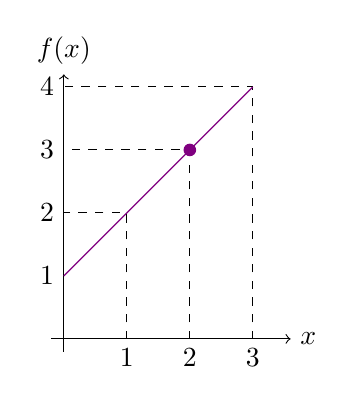
\begin{tikzpicture}[scale=0.8]
    \draw[->] (-0.2,0) -- (3.6,0) node[right] {$x$};
    \draw[->] (0,-0.2) -- (0,4.2) node[above] {$f(x)$};
    %
    \draw[dashed] (0,0) -- (0,1) node[left]{$1$};
    \draw[dashed] (1,0) node[below]{$1$} -- (1,2) -- (0,2) node[left]{$2$};
    \draw[dashed] (2,0) node[below]{$2$} -- (2,3) -- (0,3) node[left]{$3$};
    \draw[dashed] (3,0) node[below]{$3$} -- (3,4) -- (0,4) node[left]{$4$};
    %
    \draw[violet] (0,1) -- (3,4);
    \fill[violet] (2,3) circle[radius=1mm];
\end{tikzpicture}%Also used by abbildungen/04_abbildungen_in_koordinatensystemen
    }
    Der rechts abgebildete Graph gehört zur Abbildung \mbox{$f(x)=x+1$}. Der eingezeichnete Punkt hat die $x$-Koordinate $2$ und damit insgesamt die Koordinate $\coord{2}{f(2)}=\coord{2}{3}$. 
    
    Weil jedes Argument nur ein Bild haben kann, gibt es nur einen Punkt auf dem Graph von $f$, der den $x$-Wert $2$ hat.
    
    \picskip{3}
    Der Graph schneidet die $y$-Achse beim Wert $1$. Der dort liegende Punkt hat die $x$-Koordinate $0$ und insgesamt die Koordinate $\coord{0}{f(0)}=\coord{0}{1}$. Damit hat die Abbildung $f$ den $y$-Achsenabschnitt $1$.
    
    Der $y$-Achsenabschnitt von $f$ entspricht somit dem Wert $f(0)$ -- denn auf genau dieser Höhe liegt der Punkt über $x=0$, der die entsprechende Abbildungsvorschrift darstellt.
\end{example}

Um einen Abbildungsgraphen zu erhalten, hatten wir über jedem möglichen Argument (also jedem möglichen $x$-Wert) einen Punkt eingezeichnet. Jeder Punkt auf dem Abbildungsgraph steht für eine Abbildungsregel, die ein bestimmtes Argument auf ein bestimmtes Bild abbildet und hat die Koordinate $\coord{x}{f(x)}$ für ein $x\in\Real$.

Wir suchen nun einen Punkt, der auf dem Graphen einer Abbildung und gleichzeitig auch auf der $y$-Achse liegt. Jeder Punkt, der auf der $y$-Achse liegt, hat den $x$-Wert $0$ (die $y$-Achse geht nämlich vom Ursprung, dessen Koordinate $\coord{0}{0}$ ist, gerade nach oben und hat deshalb denselben $x$-Wert wie der Ursprung). 

Im Beispiel haben wir bereits gesehen, dass $\coord{0}{f(0)}$ der einzige Punkt auf dem Graphen ist, der auf der $y$-Achse liegt. Um den $y$-Achsenabschnitt einer beliebigen Abbildung auszurechnen, genügt es aus diesem Grund, einfach $f(0)$ zu berechnen.

\begin{example}{}
    \sloppy
    Die Abbildung $f(x)=4(x+1)$ hat den $y$-Achsenabschnitt $4$, denn um den $y$-Achsenabschnitt zu berechnen, muss einfach nur $f(0)$ berechnet werden. Es gilt $f(0)=4\cdot (0+1)=4$.
\end{example}

\fussy

\subsection{Nullstellen}
\label{sec:abbildungen_nullstelle}

Wie bereits beim $y$-Achsenabschnitt ist es, wenn man einen Graphe sieht, natürlich möglich, durch Hinsehen zu bestimmen, wo der Graph die $x$-Achse schneidet -- allerdings auch hier mit denselben Problemen. Um also zu \emph{berechnen}, wo ein Abbildungsgraph die $x$-Achse schneidet, müssen Punkte berechnet werden, deren $y$-Koordinate $0$ ist (das ist die Bedingung dafür, dass ein Punkt auf der $x$-Achse liegt).

Jeder Punkt auf dem Abbildungsgraphen hat die Koordinate $\coord{x}{f(x)}$, also eine Kombination aus einem Element $x$ aus der Definitionsmenge und dem Bild $f(x)$, auf das $x$ abgebildet wird. Damit die $y$-Koordinate $0$ wird, muss der rechte Teil, also $f(0)$, null werden. Für Schnittpunkte mit der $x$-Ache müssen deshalb einfach Werte für $x$ gefunden werden, für die $f(x)=0$ gilt.

\begin{example}{}
    \parpic[r]{
        \begin{tikzpicture}[samples=\ifdraft{5}{30}]
            \begin{axis}[defgrid, domain=0:4, y=.75cm, x=.75cm, xtick={1,...,4}, ytick={-1,...,3}, samples=\ifdraft{5}{20}]
                \addplot[color=violet] expression{(x-2)^2-1};
            \end{axis}
        \end{tikzpicture}
    }
    Rechts ist der Graph der Abbildung $f(x)=(x-2)^2-1$ abgebildet. Der Graph schneidet die $x$-Achse bei $x=1$ und $x=3$. 
    
    Das liegt daran, dass die Abbildung für beide $x$-Werte null wird: Es gilt \[f(3)=(3-2)^2-1=1-1=0\] und \[f(1)=(1-2)^2-1=1-1=0.\]
    
    \picskip{0}
    Wie du darauf kommen kannst, dass die Abbildung ausgerechnet an den Stellen $1$ und $3$ den Wert $0$ annimmt, ist zunächst nicht wichtig (das wird Gegenstand der Kapitel über lineare und quadratische Gleichungen sein).
    
    Weil der $y$-Wert eines Punktes auf dem Graphen immer $f(x)$ (also dem Bild eines gewissen Arguments) entspricht, ist liegt für diese beiden $x$-Werte der Punkt auf der $x$-Achse (denn der $y$-Wert ist $0$).
\end{example}

Der Graph einer Abbildung schneidet die $x$-Achse immer dann, wenn das Bild des betreffenden $x$-Wertes $0$ ist, also wenn $f(x)=0$ gilt. Wegen dieser Eigenschaft nennt man die $x$-Werte, für die eine Abbildung den Wert $0$ annimmt (und damit die $x$-Achse schneidet) auch \textbf{Nullstellen}.

\begin{definition}{Nullstelle\index{Nullstelle}}
    Ist $f$ eine Abbildung, dann heißen alle $x\in\Real$ mit $f(x)=0$ \textbf{Nullstellen} von $f$.
\end{definition}

Um herauszufinden, welche Werte man für $x$ wählen kann, damit $f(x)=0$ gilt, ist es nötig, eine Gleichung aufzulösen. $f(x)$ sollte dir immer in Form einer Berechnungsvorschrift vorliegen, z.B. in der Art \enquote{$f(x)=2x$}. Nun wäre es erforderlich, die Gleichung $2x=0$ aufzulösen, also alle $x$ zu finden, für die $2x=0$ gilt. 

Das lernst du vor allem in den Kapiteln über \textbf{lineare und quadratische Gleichungen}. Zunächst wird es nicht erforderlich sein, dass du systematisch Gleichungen lösen kannst -- stattdessen werden die Nullstellen in der Regel so einfach sein, dass sie sich leicht durch Ausprobieren finden lassen.

\begin{example}{}
    Die Nullstellen der Abbildung $f(x)=x+5$ sind alle Werte, die sich für $x$ einsetzen lassen, damit $f(x)=0$ gilt. Es muss die Gleichung $\colorbrace{x+5}{f(x)}=0$ gelöst werden. Der einzige Wert, den man für $x$ wählen kann, damit $f(x)=x+5=0$ gilt, ist $x=-5$.
    
    Es folgt, dass $f$ genau eine Nullstelle hat, und zwar bei $x=-5$.
\end{example}

\begin{nutshell}{Nullstellen und $y$-Achsenabschnitt}
    Die Schnittpunkte eines Abbildungsgraphen mit den beiden Koordinatenachsen (also der $x$-Achse und der $y$-Achse) werden besonders bezeichnet.
    
    Ein Schnittpunkt des Graphen einer Abbildung $f$ mit der $x$-Achse wird als \textbf{Nullstelle} von $f$ bezeichnet, weil die Abbildung hier den Wert 0 hat: Damit der Graph die $x$-Achse an einem Punkt $\coord{x}{0}$ schneidet, muss $f(x)=0$ sein. Grundsätzlich kann eine Abbildung mehrere Nullstellen haben, nämlich dann, wenn es mehrere verschiedene Werte für $x$ gibt, sodass $f(x)=0$ gilt.
    
    Ein Schnittpunkt des Graphen von $f$ mit der $y$-Achse heißt \textbf{$y$-Achsenabschnitt} von $f$. Jede Abbildung hat nur einen $y$-Achsenabschnitt, weil jeder Punkt auf der $y$-Achse eine Koordinate $\coord{0}{y}$ haben muss, deren $x$-Wert 0 ist. Der $y$-Achsenabschnitt ist genau der Wert $f(0)$, weil das die einzige Abbildungsregel ist, die einen Punkt auf der $y$-Achse erzeugen kann.
\end{nutshell}

\subsection{Monotonieverhalten}
\label{sec:abbildungen_monotonie}

Was kann mit den Funktionswerten einer Abbildung passieren, wenn man größere Argumente einsetzt?

Eine sehr spezielle und auch eher uninteressante Art von Abbildungen sind solche, deren Abbildungsvorschrift jedem beliebigen Argument das gleiche Bild zuordnet. Abbildungen, die diese Eigenschaft haben, heißen \textbf{konstant}.

\begin{example}{}
    \parpic[r]{
        \begin{tikzpicture}
            \begin{axis}[defgrid, domain=0:3, y=.8cm, x=.8cm, ymin=0, ymax=2, samples=2, ylabel=$f(x)$, xlabel=$x$]
                \addplot[color=violet] expression{2};
            \end{axis}
        \end{tikzpicture}
    }
    
    Die Abbildung $f(x)=2$ ordnet jeder beliebigen Zahl den Wert $2$ zu. Das Bild, das $f$ produziert, hängt also überhaupt nicht davon ab, welches Argument in die Abbildung eingesetzt wird. Deshalb ist $f$ eine \emph{konstante} Abbildung.
    
    Der Graph von $f$ ist eine horizontale Linie. Die Linie verläuft immer auf der Höhe des Bildes, auf das die Abbildung ihre Argumente abbildet. Weil dieses Bild immer dasselbe ist, ist auch die $y$-Koordinate von jedem Punkt auf dem Graphen dieselbe. Daher kommt die horizontale Linie.
\end{example}

Die Funktionswerte von konstanten Abbildungen verändern sich nicht, wenn man das Argument ändert. Sie bleiben also immer gleich, wenn man größere Argumente einsetzt.

Spannender sind natürlich Abbildungen, die auch verschiedene Funktionswerte annehmen können. Wenn man den Graphen einer Abbildung nach rechts verfolgt, können im Wesentlichen vier verschiedene Dinge passieren:
\begin{itemize}
    \item Der Abbildungsgraph bleibt konstant auf einer Höhe (wie im letzten Beispiel)
    \item Der Abbildungspgrah steigt immer weiter nach oben, wenn man ihm nach rechts folgt (d.h. wenn man größere Argumente $x$ in die Abbildung einsetzt, wird auch ihr Funktionswert größer)
    \item Der Abbildungspgrah fällt immer weiter nach unten, wenn man ihm nach rechts folgt (d.h. wenn man größere Argumente $x$ in die Abbildung einsetzt, wird ihr Funktionswert kleiner)
    \item Der Abbildungsgraph führt in keine klare Richtung, sondern mal nach oben, mal nach unten (d.h. wenn man größere Argumente $x$ in die Abbildung einsetzt, kann man nicht vorher sagen, ob der Funktionswert größer oder kleiner wird)
\end{itemize}

Den Fall konstanter Abbildungen haben wir im letzten Beispiel gesehen. Im folgenden Bild siehst du, wie ein Abbildungsgraph in den anderen drei Fällen beispielsweise aussehen kann.

\begin{figure}[ht]
    \centering
    \begin{multicols}{3}\centering
        \begin{tikzpicture}[samples=40]
            \begin{axis}[defgrid, domain=0:4, y=.75cm, x=.75cm, ymin=-1, ymax=3, xtick={1,...,4}, ytick={1,2,3}, samples=\ifdraft{5}{17}]
                \addplot[color=violet] expression{sqrt(x)-0.5};
            \end{axis}
        \end{tikzpicture}
        \begin{tikzpicture}[samples=2]
            \begin{axis}[defgrid, domain=0:4, y=.75cm, x=.75cm, ymin=-1, ymax=3, xtick={1,...,4}, ytick={1,2,3}, samples=2]
                \addplot[color=violet] expression{3-0.875*x};
            \end{axis}
        \end{tikzpicture}
        \begin{tikzpicture}[samples=40]
            \begin{axis}[defgrid, domain=0:4, y=.75cm, x=.75cm, ymin=-1, ymax=3, xtick={1,...,4}, ytick={1,2,3}, samples=\ifdraft{7}{40}]
                \addplot[color=violet] expression{sin(4*deg(x))};
            \end{axis}
        \end{tikzpicture}
    \end{multicols}
    \caption{Im linken Beispiel steigt der Abbildungsgraph nach rechts hin immer weiter. Im mittleren Beispiel fällt er immer weiter. Beide Graphen steigen bzw. sinken ohne Unterbrechung, d.h. sie wechseln nicht zwischendurch die Richtung. Dies ist eine besondere Eigenschaft, denn für Argumente $x$ und $y$ mit $x<y$ gilt im linken Beispiel immer $f(x)<f(y)$. Im mittleren Bild gilt stattdessen immer $f(x)>f(y)$, denn die Funktionswerte werden dort immer kleiner.
    Schließlich lässt sich für die rechts dargestellte Abbildung keine solche Aussage treffen: Je nachdem, \emph{wie weit} man nach rechts geht, kann es sowohl sein, dass man einen größeren Wert erreicht als auch, dass man einen kleineren erreicht.}
    %\label{fig:my_label}
\end{figure}

Eine Abbildung, deren Graph dauerhaft fällt oder dauerhaft sinkt, heißt \textbf{monoton}. Das bedeutet, dass der Graph seine Richtung (entweder nach oben oder nach unten) nicht ändert. Die beiden links abgebildeten Graphen im obigen Bild gehören somit zu einer monotonen Abbildung. Sie führen entweder konsequent nur nach oben (links) oder konsequent nur nach unten (Mitte).

\begin{definition}{Monotonie\index{Monotonie}}
    Eine Abbildung $f$ heißt \textbf{monoton steigend}, falls $f(x)\leq f(y)$ für alle $x<y$ gilt. Sie heißt \textbf{streng monoton steigend}, falls $f(x)<f(y)$ für alle $x<y$ gilt.
    
    Analog heißt sie \textbf{monoton fallend}, falls $f(x)\geq f(y)$ für alle $x<y$ gilt und \textbf{streng monoton fallend}, falls $f(x)>f(y)$ für alle $x<y$ gilt.
    
    Eine Abbildung, die entweder monoton fallend oder monoton steigend ist, heißt \textbf{monoton}.
\end{definition}

Bei strenger Monotonie muss ein Graph tatsächlich pausenlos steigen, die Funktionswerte müssen also wirklich immer größer werden (im Falle von streng monoton steigend, bei streng monoton fallend ist es genau umgekehrt). Damit eine Abbildung nur monoton steigend ist, reicht es, wenn sie nicht zwischendurch fällt. Schaust du dir den Abbildungsgraphen an, musst du also bei strenger Monotonie darauf achten, ob der Graph zwischendurch konstant ist. Nur wenn es keine konstanten Stellen gibt, ist eine Abbildung wirklich \emph{streng} monoton.

Wenn bestimmt werden soll, ob eine Abbildung monoton ist, dann lässt sich das anhand ihres Abbildungsgraphen ablesen: Wenn dieser stets steigt (dann ist die Abbildung streng monoton steigend) oder stets fällt (streng monoton fallend), dann ist der Fall klar. Gibt es ein auf- und ab, dann ist die Abbildung nicht monoton. Wenn der Graph zwar nicht dauerhaft steigt, aber zumindest nie sinkt, dann ist die Abbildung immerhin noch monoton steigend (aber nicht mehr streng monoton steigend). Genauso funktioniert das, wenn die Abbildung nie steigt: Dann ist sie monoton fallend. 

Es ist auch möglich, Monotonie rechnerisch nachzuweisen. Wirklich adäquate Mittel dafür erlernst du allerdings erst im Kapitel über \textbf{Differentialrechnung in \Real}.\todocomment{Hier am besten eine verlinkung}

\begin{example}{}
    
    \parpic[r]{
        \begin{tikzpicture}
            \begin{axis}[defgrid, domain=0:4, y=.5cm, x=.75cm, xtick={1,...,4}, ytick={1,2,3}, samples=2]
                \addplot[color=violet] expression{3-x};
            \end{axis}
        \end{tikzpicture}
    }
    
    Die Abbildung $f(x)=3-x$ ist streng monoton fallend, weil die Funktionswerte kleiner werden, je größer das $x$ wird (denn man zieht dann immer größere Zahlen von der Zahl $3$ ab). Wie bei jeder streng monoton fallenden Abbildung sieht man auch, dass der Graph stetig nach unten führt.
    
    \parpic[r]{
        \begin{tikzpicture}
            \begin{axis}[defgrid, domain=0:4, y=.5cm, x=.75cm, ymin=0, xtick={1,...,4}, ytick={1,2,3}, samples=2]
                \addplot[color=violet] expression{2};
            \end{axis}
        \end{tikzpicture}
    }
    
    Die Abbildung $f(x)=2$ ist monoton steigend und monoton fallend, weil jeweils \mbox{$f(x)=f(y)$} für alle $x,y\in\Real$ gilt. Deshalb gilt insbesondere auch $f(x)\leq f(y)$ und $f(x)\geq f(y)$ für alle $x,y$. Sie ist allerdings nicht streng monoton steigend oder fallend, weil die Funktionswerte nicht tatsächlich größer oder kleiner werden.
\end{example}

\begin{nutshell}{Monotonie}
    Man spricht davon, dass eine Abbildung \textbf{monoton} ist, wenn ihre Funktionswerte für steigende Argumente $x$, die man in die Abbildung einsetzt, entweder niemals größer werden oder niemals kleiner werden.
    
    Eine Abbildung $f$ heißt \textbf{monoton steigend}, falls $f(x)\leq f(y)$ für alle $x<y$ gilt, also wenn ihre Funktionswerte für steigende Argumente $x$ nicht kleiner werden. Entsprechend heißt sie \textbf{monoton fallend}, wenn ihre Funktionswerte für steigende $x$ nicht größer werden, also $f(x)\geq f(y)$ für alle $x<y$.
    
    Eine Abbildung heißt bereits dann monoton steigend, wenn sie nie fällt. Es ist allerdings erlaubt, dass sie konstant bleibt. Wenn eine Abbildung tatsächlich dauerhaft steigt und nie konstant bleibt, dann heißt sie \textbf{streng monoton steigend}. Es gilt dann $f(x)<f(y)$ für alle $x<y$. Wenn eine Abbildung stattdessen dauerhaft sinkt, dann heißt sie \textbf{streng monoton fallend} und es gilt $f(x)>f(y)$ für alle $x<y$.
\end{nutshell}

\subsection{Symmetrien des Abbildungsgraphen}
\label{sec:abbildungen_symmetrie}

Die wichtigsten Symmetrien, die du aus den Grundlagen der Geometrie kennst, sind Spiegelungen und Drehungen. Nachfolgend geht es darum, Spiegelungen bei Abbildungsgraphen zu suchen.

Wenn man davon spricht, dass der Graph einer Abbildung symmetrisch ist, dann meint man normalerweise \enquote{symmetrisch am Ursprung} oder \enquote{symmetrisch an der $y$-Achse}. Prinzipiell heißt das, dass der Graph links von der $y$-Achse auf die gleiche Weise verläuft wie rechts von der $y$-Achse.

\begin{advanced}{Symmetrien}
    Man kann auch allgemeiner Symmetrien statt nur Spiegelungen bei Abbildungsgraphen suchen. Eine \textbf{Symmetrie} ist eine Abbildung, die die Punkte einer geometrischen Figur (also zum Beispiel die Punkte auf einem Abbildungsgraphen) umordnet und dabei Abstände beibehält. Zwei Punkte, die einen Abstand von 1 haben, müssen durch eine Symmetrie demnach auf zwei Punkte abgebildet werden, deren Abstand ebenfalls 1 ist.
    
    \begin{definition}{Symmetrie}
        Es sei $F$ eine geometrische Figur, dargestellt durch die Menge der Punkte, die zur Figur gehören. Dann heißt eine bijektive Abbildung $s\colon F\rightarrow F$ eine Symmetrie von $F$, falls beliebige $f_1,f_2\in F$ stets denselben Abstand wie $s(f_1)$ und $s(f_2)$ haben.
    \end{definition}
    
    \begin{advexample}{}
        \parpic[r]{
            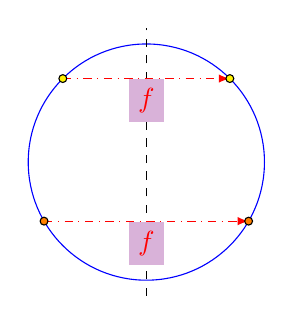
\begin{tikzpicture}
                \draw[blue] (0,0) circle[radius=1.5cm];
                \draw[dashed] (0,-1.7) -- (0,1.7);
                \draw[-latex,dash dot,red] (135:1.5) -- node[fill=violet!30,below] {$f$} (45:1.5);
                \draw[-latex,dash dot,red] (-150:1.5) -- node[fill=violet!30,below] {$f$} (-30:1.5);
                \draw[fill=yellow] (45:1.5) circle[radius=.5mm];
                \draw[fill=yellow] (135:1.5) circle[radius=.5mm];
                \draw[fill=orange] (-30:1.5) circle[radius=.5mm];
                \draw[fill=orange] (-150:1.5) circle[radius=.5mm];
            \end{tikzpicture}
        }
        Eine Symmetrie des rechts abgebildeten blauen Kreises ist die eingezeichnete Abbildung, die jeden Punkt des Kreises an der gestrichelt eingezeichneten Spiegelachse spiegelt.
        
        Nach der Anwendung der Spiegelung erhält man d\textbf{en gleichen Kreis wie vorher}. Außerdem haben zwei Punkte vor der Spiegelung immer den \textbf{gleichen Abstand} wie nach der Spiegelung. Diese beiden Eigenschaften machen die eingezeichnete Abbildung zu einer Symmetrie.
        
        Eine weitere Symmetrie des Kreises ist eine Abbildung, die jeden Punkt auf sich selbst abbildet. Diese Symmetrie existiert bei jeder geometrischen Figur und behält natürlich auch die Abstände bei, weil sie die Punkte nicht verschiebt.
    \end{advexample}
\end{advanced}

\begin{example}{}
    \parpic[r]{
        \begin{tikzpicture}
            \begin{axis}[defgrid, domain=-2:2, y=.75cm, x=.75cm, xtick={-2,...,2}, ytick={1,2,3}, samples=\ifdraft{5}{20}]
                \addplot[color=violet] expression{x^2-1};
            \end{axis}
        \end{tikzpicture}
    }
    Der rechts abgebildete Graph, der durch die Berechnungsvorschrift $f(x)=x^2-1$ entsteht, verläuft links von der $y$-Achse genauso wie rechts von von der $y$-Achse: Egal, ob man dem Graphen von der $y$-Achse nach links oder rechts folgt, seine $y$-Werte entwickeln sich immer gleich.
    
    Man sieht, dass der Graph achsensymmetrisch an der $y$-Achse ist (man nutzt die $y$-Achse also als Spiegelachse).
\end{example}

Der Graph aus dem letzten Beispiel ist \textbf{achsensymmetrisch an der $y$-Achse}. Das heißt, dass die $y$-Achse als Spiegelachse fungiert und sich der Teil links von der $y$-Achse auf den Teil rechts von der $y$-Achse klappen lässt.

\begin{figure}[ht]
    \centering
    \begin{tikzpicture}
        \begin{axis}[defgrid, domain=-2:2, y=0.9cm, x=0.9cm, xtick={-2,...,2}, ytick={1,2,3}, ymax=3]
            \addplot[mark=*, only marks, fill=white] coordinates {(-1,2) (1, 2)};
            \addplot[mark=*, only marks, fill=yellow] coordinates {(-2,1) (2, 1)};
            \draw[-latex,red,dashed] (-2,1) to[bend left] (2,1);
            \draw[-latex,red,dashed] (-1,2) to[bend left] (1,2);
        \end{axis}
    \end{tikzpicture}
    \caption{Nutzt man die $y$-Achse als Spiegelachse, dann werden alle Punkte auf der linken Seite (also mit negativen $x$-Werten) in gerader Linie nach rechts gespiegelt. Der gelbe Punkt auf der linken Seite wird in waagerechter Linie nach rechts gespiegelt. Dadurch verändert sich sein $y$-Wert nicht. Durch die Spiegelung ändert sich das Vorzeichen der $x$-Koordinate, weil der Punkt nach der Spiegelung genauso weit rechts von der $y$-Achse ist wie er vorher links war.}
\end{figure}

Das bedeutet auch, dass man die gleichen Funktionswerte erhält, egal ob man von der $y$-Achse eine gewisse Schrittzahl nach links oder rechts geht: Letztendlich verläuft der Graph auf beiden Seiten auf der gleichen Höhe.

\begin{example}{}
    \parpic[r]{
        \begin{tikzpicture}
            \begin{axis}[defgrid, domain=-2:2, y=.75cm, x=.75cm, xtick={-2,...,2}, ytick={1,2}, samples=\ifdraft{5}{20}]
                \addplot[color=violet] expression{x^2-1};
                \addplot[mark=*, only marks, fill=white] coordinates {(-1,0) (1, 0)};
                \addplot[mark=*, only marks, fill=yellow] coordinates {(-2,3) (2, 3)};
                \draw[-latex,dashed,red] (-2,3) -- (2,3);
            \end{axis}
        \end{tikzpicture}
    }
    Geht man im letzten Beispiel vom Ursprung einen Schritt auf der $x$-Achse nach links, so schneidet der Graph dort beim Punkt $\coord{-1}{0}$ die $x$-Achse (dargestellt durch weiße Punkte, es gilt $f(-1)=0$). Wenn du dir vorstellst, dass du den Punkt $\coord{-1}{0}$ nun nach rechts spiegelst, dann bekommst du den Punkt $\coord{1}{0}$, der ebenfalls auf dem Graphen liegt. Dieser Punkt stellt die Regel $f(1)=0$ dar.
    
    \picskip{0}
    Wenn man zwei Schritte nach links oder rechts geht (also zu $x=-2$ oder $x=2$), dann findet man für jeden dieser $x$-Werte einen Punkt auf dem Graphen (dargestellt durch die gelben Punkte). Die Punkte haben die Koordinaten $\coord{-2}{3}$ und $\coord{2}{3}$, stellen also die Abbildungsregeln $f(-2)=3$ und $f(2)=3$ dar.
\end{example}

Im letzten Beispiel konnte beobachtet werden, dass ein beliebiger Punkt $\coord{x}{y}$ auf dem Graphen bei der Achsenspiegelung an der $y$-Achse auf den Punkt $\coord{-x}{y}$ gespiegelt wird. Das heißt, dass zu einem Graphen, der achsensymmetrisch an der $y$-Achse ist und den Punkt $\coord{x}{y}$ enthält, auch immer der Punkt $\coord{-x}{y}$ gehören muss.

Wenn der Punkt $\coord{x}{y}$ auf dem Graphen einer Abbildung liegt, dann steht das immer für die Abbildungsregel $f(x)=y$. Der gespiegelte Punkt steht also für die Regel $f(-x)=y$. Damit ist insgesamt $f(x)=f(-x)$ (denn beides hat denselben Wert, nämlich $y$). Abbildungen, deren Graph achsensymmetrisch an der $y$-Achse ist, haben also die Eigenschaft, dass $f(x)=f(-x)$ ist.

\begin{theorem}{}
    Der Graph einer Abbildung $f$ ist genau dann achsensymmetrisch an der $y$-Achse, wenn $f(x)=f(-x)$ für alle $x\in\Real$ gilt.
\end{theorem}

\begin{example}{}
    Es lässt sich rechnerisch erklären, dass der Graph der Abbildung $f(x)=x^2-1$ achsensymmetrisch an der $y$-Achse ist: Es gilt \[f(-x)=(-x)^2-1=x^2-1=f(x),\] also insgesamt $f(x)=f(-x)$. Die Bedingung $f(x)=f(-x)$ ist nach den vorherigen Überlegungen genau die Voraussetzung für die Achsensymmetrie an der $y$-Achse.
\end{example}

Anders als in den vorherigen Beispielen ist es auch möglich, dass der Graph nicht an der $y$-Achse achsengespiegelt ist, sondern stattdessen punktgespiegelt am Ursprung. Dabei wird der Graph nicht einfach von links nach rechts geklappt.

\begin{example}{}
    \parpic[r]{
        \begin{tikzpicture}
            \begin{axis}[defgrid, domain=-2:2, y=.75cm, x=.75cm, xtick={-2,...,2}, ytick={-4,...,4}, samples=\ifdraft{5}{20}]
                \addplot[color=violet] expression{0.5*x^3};
                \addplot[mark=*, only marks, fill=white] coordinates {(-1.5,-1.6875)};
                \addplot[mark=*, only marks, fill=yellow] coordinates {(1.5, 1.6875)};
                \draw[dashed,-latex] (-1.5,-1.6875) -- (1.5,1.6875);
            \end{axis}
        \end{tikzpicture}
    }
    Der Graph, den du rechts siehst, ist punktsymmetrisch. Spiegelt man zum Beispiel den weiß eingezeichneten Punkt, der bei der $x$-Koordinate $-\frac{3}{2}$ liegt, am Ursprung, dann landet man beim gelb eingezeichneten Punkt genau auf der anderen Seite.
    
    Auf die gleiche Weise wie den weißen Punkt könnte man jeden anderen Punkt vom Graphen am Ursprung spiegeln und würde jedes Mal wieder auf dem Graphen landen.
    
    War der Punkt vor der Punktspiegelung links von der $y$-Achse, so ist er anschließend rechts. Die $x$-Koordinate verändert sich wie bereits bei der Achsenspiegelung nur, indem es aus positiven Koordinaten negative werden und umgekehrt.
\end{example}

Die Punktspiegelung am Ursprung ähnelt sehr der Achsenspiegelung an der $y$-Achse: Bei der Spiegelung werden Punkte von links nach rechts (oder umgekehrt) gespiegelt. Der wesentliche Unterschied ist allerdings, dass die Spiegelung vorher in einer waagerechten Linie erfolgt ist. Hatte ein Punkt vor der Achsenspiegelung zum Beispiel die $y$-Koordinate $6$, so behält er diese Koordinate auch nach der Spiegelung.

Das ist nun anders: Punkte werden hier auch nach oben (oder unten, falls sie bereits oben waren) gespiegelt. Dadurch verändert sich bei der Spiegelung nun nicht nur die $x$-Koordinate, sondern dasselbe passiert nun auch mit der $y$-Koordinate.

Spiegeln wir etwa den Punkt $\coord{-2}{-2}$ am Ursprung, dann liegt der gespiegelte Punkt anschließend genauso weit rechts und oben wie der ursprüngliche Punkt links und unten lag. Mit anderen Worten: Bei der $x$- und der $y$-Koordinate ändert sich jeweils das Vorzeichen. Der neue Punkt lautet in diesem Fall $\coord{2}{2}$.

Liegt nun ein Punkt $\coord{x}{y}$ auf dem Abbildungsgraphen (das stellt die Regel $f(x)=y$ dar), dann liegt ebenso sein gespiegelter Punkt auf dem Graphen. Dieser hat nach den vorherigen Überlegungen die Koordinaten $\coord{-x}{-y}$ und stellt damit die Abbildungsregel $f(-x)=-y$ dar. Für jede Abbildungsregel $f(x)=y$ lässt sich demnach sofort feststellen, dass auch $f(-x)=-y$ eine Regel sein muss (denn der entsprechende Punkt liegt auf dem Graphen). Formen wir diese Bedingung ein wenig um, dann erhalten wir \[f(x)=y=-(-y)=-f(-x),\]
also hat eine Abbildung einen punktsymmetrischen Graphen, falls stets $f(x)=-f(-x)$ gilt.

\begin{theorem}{}
    Der Graph einer Abbildung $f$ ist genau dann punktsymmetrisch am Ursprung, wenn $f(x)=-f(-x)$ für alle $x\in\Real$ gilt.
\end{theorem}

\begin{example}{}
    Der Graph der Abbildung $f(x)=x^3$ ist punktsymmetrisch am Ursprung. Um zu prüfen, ob der Graph punktsymmetrisch ist, muss geschaut werden, ob \mbox{$f(x)=-f(-x)$} gilt. Weil $f(x)$ nichts anderes als $x^3$ ist, muss hier lediglich geprüft werden, ob $x^3$ dasselbe ist wie $-\colorbrace{(-x)^3}{f(-x)}$. Wir können nun leicht nachrechnen, dass
    \[-(-x)^3=-(-x^3)=x^3\]
    gilt. Und das ist genau dasselbe wie $f(x)$. Der Graph der Funktion ist also punktsymmetrisch am Ursprung.
\end{example}

\begin{nutshell}{Symmetrie bei Abbildungsgraphen}
    Einige Abbildungen haben Graphen, die entweder punkt-- oder achsensymmetrisch sind. Man unterscheidet zwischen Graphen, die achsensymmetrisch an der $y$-Achse sind und Graphen, die punktsymmetrisch am Ursprung sind.
    
    Bei einer \textbf{Spiegelung an der $y$-Achse} werden alle Punkte wagerecht von links nach rechts (oder andersrum) geklappt. Damit ein Graph achsensymmetrisch an der $y$-Achse ist, muss $f(x)=f(-x)$ gelten (d.h. er verläuft links der $y$-Achse ebenso wie rechts von der $y$-Achse).
    
    Für eine \textbf{Punktspiegelung am Ursprung} werden Punkte diagonal gespiegelt. Ein am Ursprung punktgespiegelter Graph verläuft links genauso wie rechts, allerdings mit einem Vorzeichenwechsel. Verläuft er links nach unten, dann verläuft der Graph rechts nach oben. Es liegt eine Punktsymmetrie am Ursprung vor, wenn $f(x)=-f(-x)$ gilt.
\end{nutshell}

\end{document}